\documentclass{article}
\usepackage[utf8]{inputenc}
\usepackage{float}
\usepackage{setspace}
\usepackage[spanish]{babel}
% Default fixed font does not support bold face
\DeclareFixedFont{\ttb}{T1}{txtt}{bx}{n}{12} % for bold
\DeclareFixedFont{\ttm}{T1}{txtt}{m}{n}{12}  % for normal
% Custom colors
\usepackage{color}
\definecolor{deepblue}{rgb}{0,0,0.5}
\definecolor{deepred}{rgb}{0.6,0,0}
\definecolor{deepgreen}{rgb}{0,0.5,0}
\usepackage{listings}

\definecolor{Code}{rgb}{0,0,0}
\definecolor{Decorators}{rgb}{0.5,0.5,0.5}
\definecolor{Numbers}{rgb}{0.5,0,0}
\definecolor{MatchingBrackets}{rgb}{0.25,0.5,0.5}
\definecolor{Keywords}{rgb}{0,0,1}
\definecolor{self}{rgb}{0,0,0}
\definecolor{Strings}{rgb}{0,0.63,0}
\definecolor{Comments}{rgb}{0,0.63,1}
\definecolor{Backquotes}{rgb}{0,0,0}
\definecolor{Classname}{rgb}{0,0,0}
\definecolor{FunctionName}{rgb}{0,0,0}
\definecolor{Operators}{rgb}{0,0,0}
\definecolor{Background}{rgb}{0.98,0.98,0.98}

\lstnewenvironment{python}[1][]{
\lstset{
numbers=left,
numberstyle=\footnotesize,
numbersep=1em,
xleftmargin=1em,
framextopmargin=2em,
framexbottommargin=2em,
showspaces=false,
showtabs=false,
showstringspaces=false,
frame=l,
tabsize=4,
% Basic
basicstyle=\ttfamily\small\setstretch{1},
backgroundcolor=\color{Background},
language=Python,
% Comments
commentstyle=\color{Comments}\slshape,
% Strings
stringstyle=\color{Strings},
morecomment=[s][\color{Strings}]{"""}{"""},
morecomment=[s][\color{Strings}]{'''}{'''},
% keywords
morekeywords={import,from,class,def,for,while,if,is,in,elif,else,not,and,or,print,break,continue,return,True,False,None,access,as,,del,except,exec,finally,global,import,lambda,pass,print,raise,try,assert},
keywordstyle={\color{Keywords}\bfseries},
% additional keywords
morekeywords={[2]@invariant},
keywordstyle={[2]\color{Decorators}\slshape},
emph={self},
emphstyle={\color{self}\slshape},
%
}}{}


\title{Tarea 3 - Redes de Computadores}
\author{Juan Carlos Arriagada 2973565-4\\Celeste Bertin 201092008-9}
\date{20 de Junio del 2014}

\usepackage{natbib}
\usepackage{graphicx}

\begin{document}

\maketitle

\section{Introducción}
El presente informe tiene por objetivo mostrar al lector cual es el camino que sigue la información para llegar a su destino, explicando brevemente porque son así las rutas. Además, se espera familiarizar al lector con el algoritmo de Vector-Distancia para calcular la ruta más corta para el envío de paquetes  y explicar cómo es que este algoritmo permite darle robustez a las redes en caso de falla de algún enlace físico.

\section{Desarrollo}
El presente informe se divide en 3 items, los cuales son ''comunicación intercontinental'', ''tabla de costo de routers'' y ''tabla de costo de routers en caso de modificación de conexiones'', los cuales se detallan a continuación:
\subsection{Comunicación Intercontinental}
Desde la creación de la telegrafía, la humanidad ha tratado de comunicarse a largas distancias de forma rápida y efectiva. Un gran desafío fue la comunicación entre continentes, para lo cual se tendió un cable de cobre entre Europa y América del Norte, logrando reducir el tiempo de envío de mensajes a unos pocos minutos, en comparación a los 10 días que tomaba enviar un mensaje por barco \citep{website:galido}. 
Hoy en día, la información viaja de forma rápida y efectiva entre continentes a través de cables submarinos de fibra óptica, los cuales transmiten las señales digitales utilizadas para telecomunicaciones internacionales, entre los cuales está el internet. Estos cables están instalados entre continentes de tal forma que si se daña alguno, existe redundancia de las conexiones tal que no se pierda comunicación en caso de contratiempos, como por ejemplo, un cable cortado. Los cables usados actualmente están compuestos de varias capas, para protección de los cables de fibra óptica los cuales son usados para el envío de información. Para transmitir información a través de tan largas distancia, se le agregan al cable repetidores cada 60 kilómetros, los cuales amplifican la señal \citep{website:cablestransoceanicos}.
En caso de dañarse el cable, una embarcación de reparación va al punto de ruptura, sube ambos extremos a la superficie y los conecta de nuevo con una extensión nueva de cable. El cable luego de ser reparado es más largo que el cable original, por ende se deja el cable en forma de ''U'' en el fondo del mar \citep{website:repair}.

Chile está conectado al resto del mundo a través de varios cables submarinos de fibra óptica \citep{website:telegeography}, los cuales son:

\begin{itemize}
  \item Panamericano (PAN-AM)
  \item South America-1 (SAm-1)
  \item South American Crossing (SAC)/Latin American Nautilus (LAN)
\end{itemize}

Los cuales se pueden ver en la siguiente figura:

\begin{figure}[H]
\centering
\setlength\fboxsep{0pt}
\setlength\fboxrule{0.5pt}
\fbox{
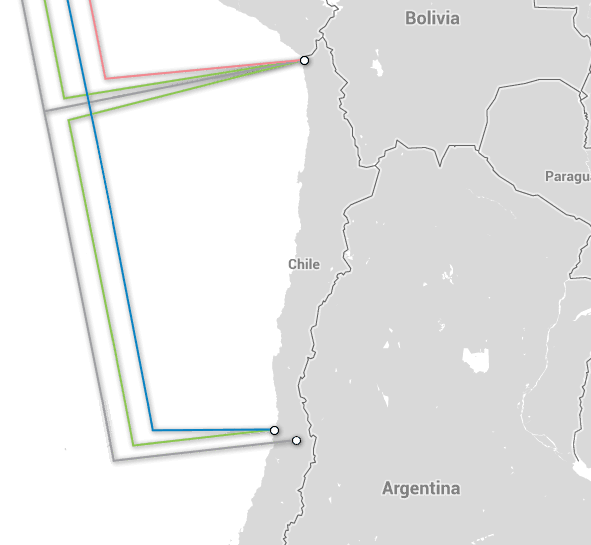
\includegraphics[scale=0.5]{underseaCable.png}}
\caption{Cables submarinos que conectan a Chile a otros continentes}
\label{fig:cables submarinos}
\end{figure}

A continuación se utiliza Open Visual Trace Route 5.1.1 para investigar la ruta tomada por los paquetes al acceder a los siguientes sitios web desde Santiago de Chile:
\clearpage

\begin{description}
\item[Moodle] \hfill \\
Se ingresó http://moodle.inf.utfsm.cl/ a Open Visual Trace Route, el cual mostró las rutas tomadas para llevar al server final. Se puede ser que el server de Moodle queda en Valparaíso. Cabe notar que si se accede a Moodle desde el internet de la Universidad misma, se accede directamente, ya que Moodle está en los servidores de la universidad.

\begin{figure}[H]
\centering
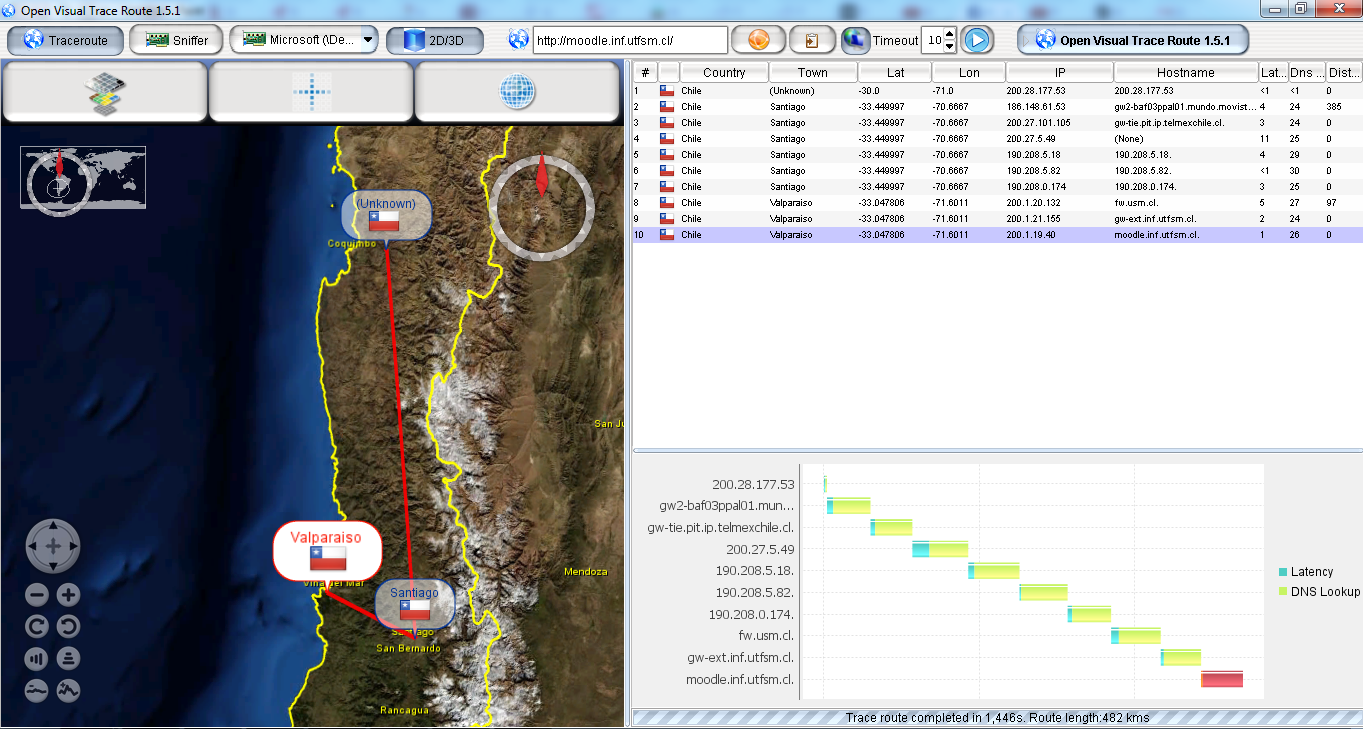
\includegraphics[width=\textwidth]{tracerouteMoodle.png}
\caption{Trace Route de moodle.inf.utfsm.cl desde Santiago}
\label{fig:moodle}
\end{figure}  

\begin{figure}[H]
\centering
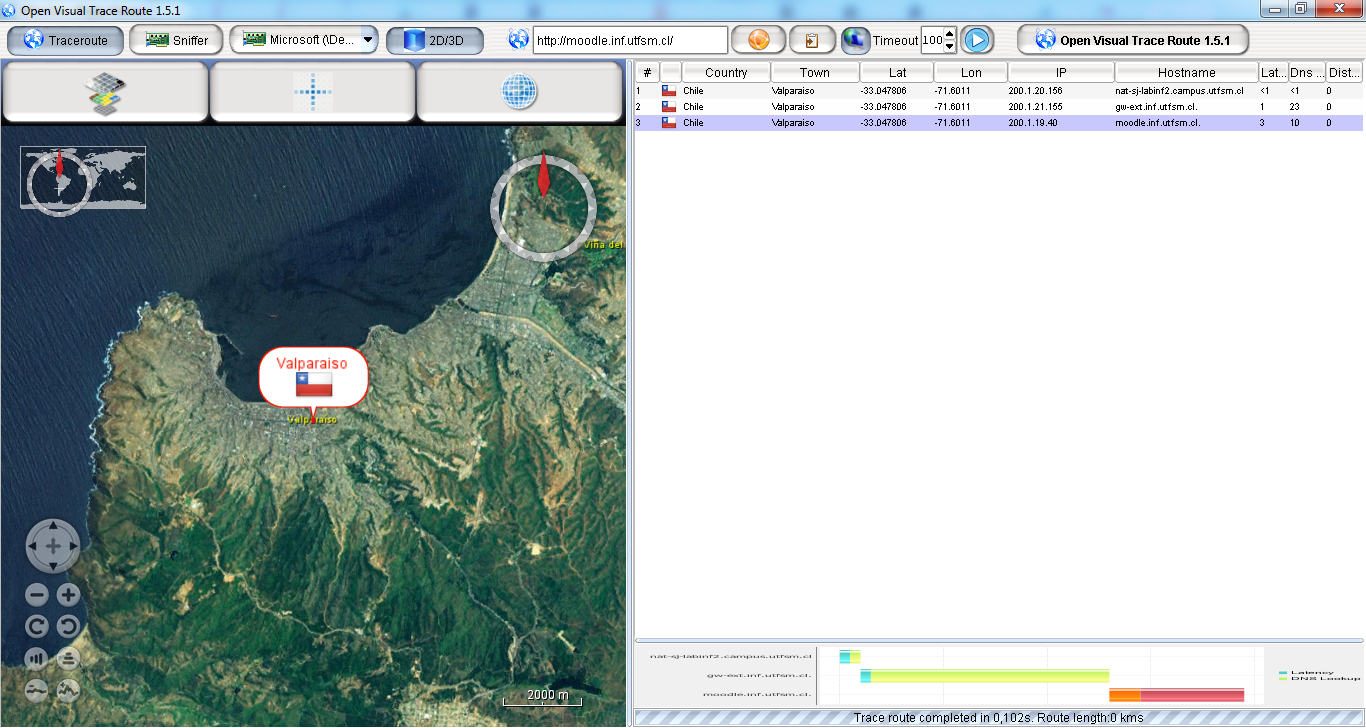
\includegraphics[width=\textwidth]{tracerouteMoodleValpo.png}
\caption{Trace Route de moodle.inf.utfsm.cl dentro de la red de la Universidad Técnica Federico Santa María}
\label{fig:moodle valparaiso}
\end{figure}  

\item[Google.cl] \hfill \\
Se ingresó http://google.cl/ a Open Visual Trace Route, el cual mostró las rutas tomadas para llevar al server final. Se puede ver que el server de Google.cl está ubicado en Mountain View, Estados Unidos, lo cual concuerda con la sede principal de Google\citep{website:google}.

\begin{figure}[H]
\centering
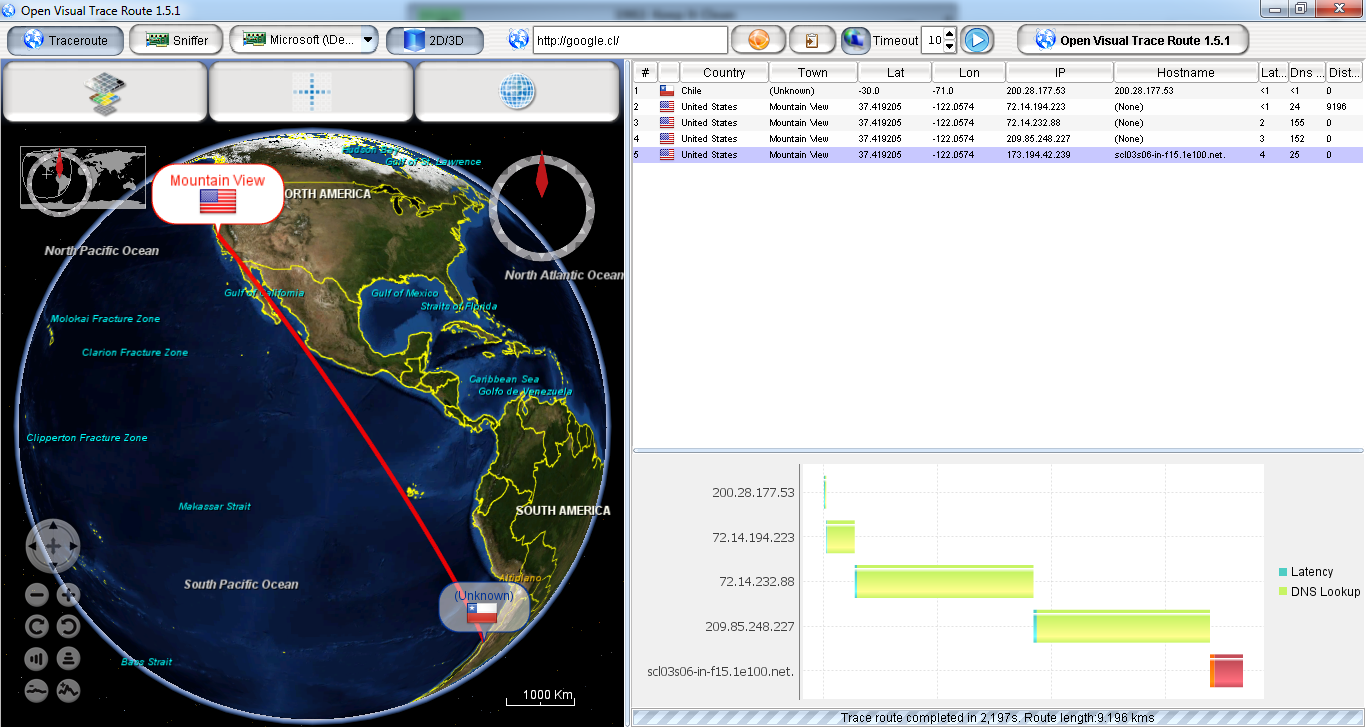
\includegraphics[width=\textwidth]{tracerouteGoogleCL.png}
\caption{Trace Route de google.cl}
\label{fig:google}
\end{figure}    
  
\item[Cime] \hfill \\
Se ingresó http://cime.cl/ a Open Visual Trace Route, el cual mostró las rutas tomadas para llevar al server final. Se puede ver que el server de Cime está en Nueva York, Estados Unidos.

\begin{figure}[H]
\centering
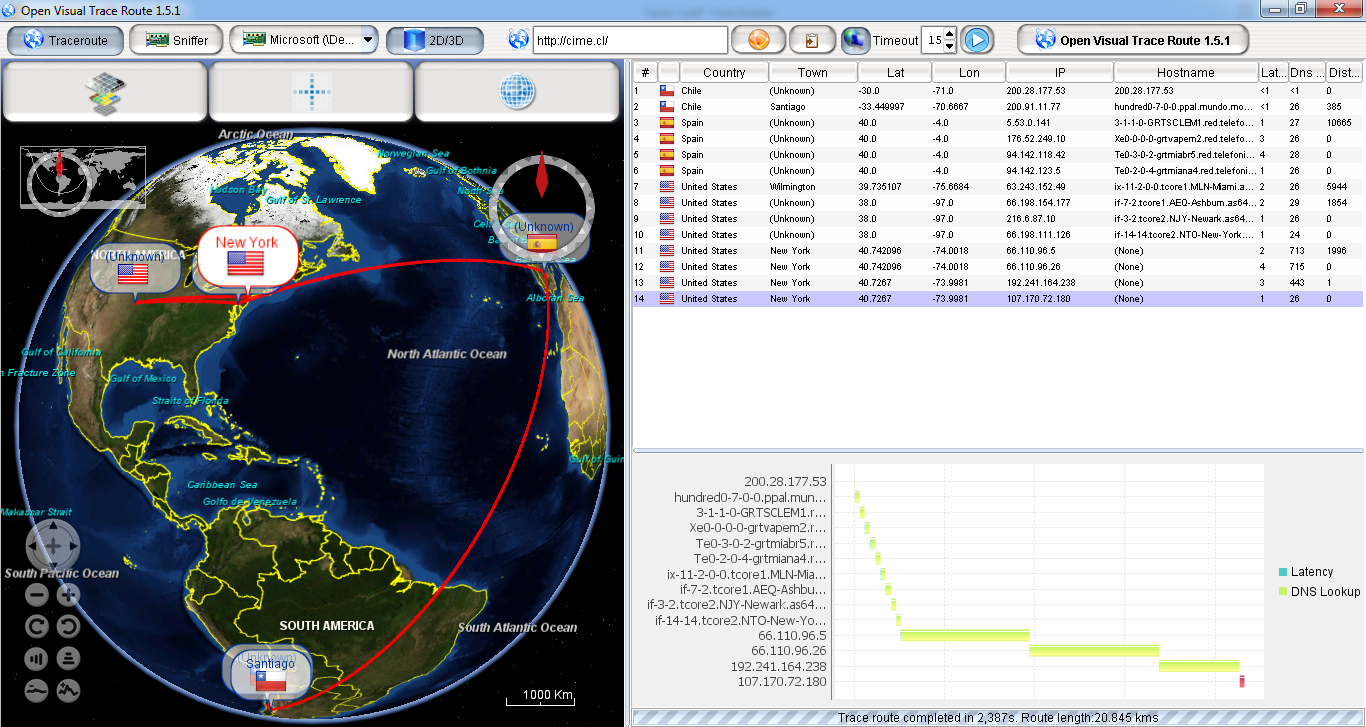
\includegraphics[width=\textwidth]{tracerouteCime.png}
\caption{Trace Route de cime.cl}
\label{fig:cime}
\end{figure}    

\item[Wikipedia] \hfill \\
Se ingresó http://wikipedia.com/ a Open Visual Trace Route, el cual mostró las rutas tomadas para llevar al server final. Se puede ver que el server de Wikipedia está en San Francisco, Estados Unidos. Esto concuerda con la localización de los servidores de Wikimedia\citep{website:wikimedia}.

\begin{figure}[H]
\centering
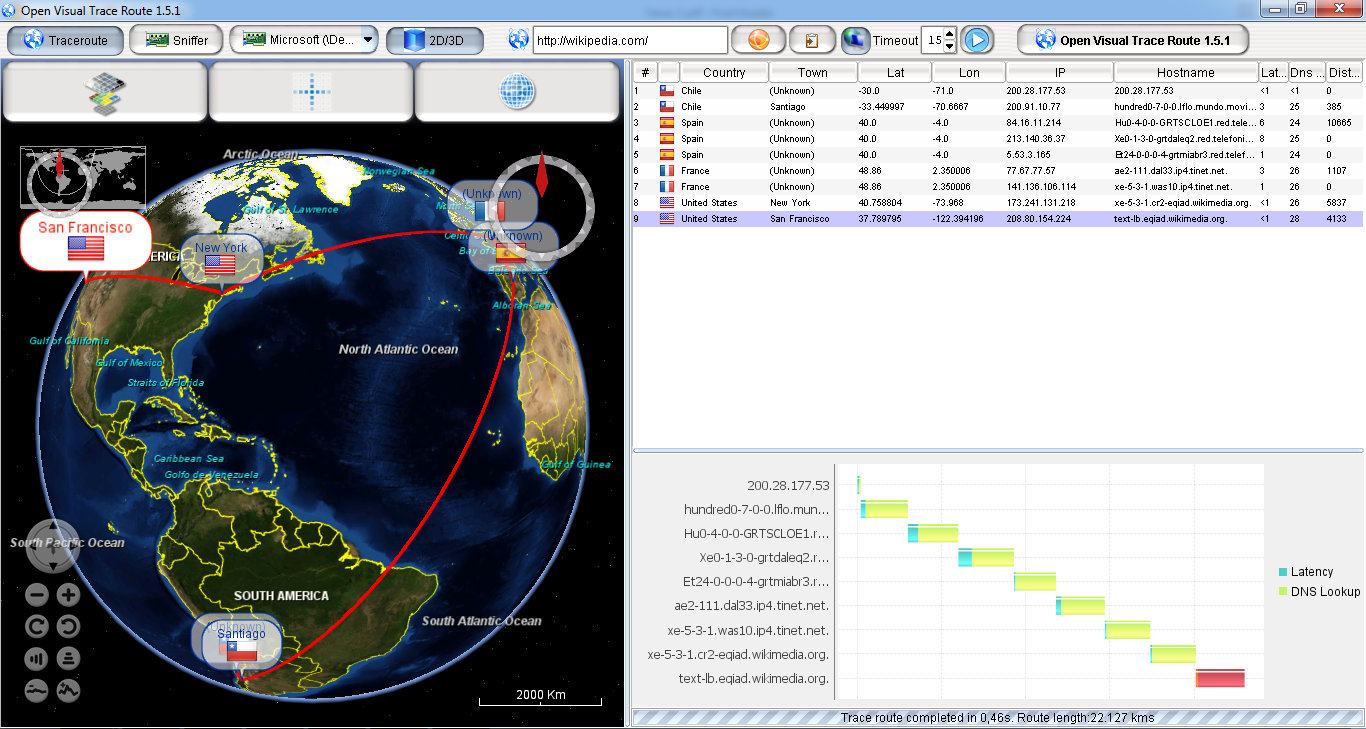
\includegraphics[width=\textwidth]{tracerouteWikipedia.png}
\caption{Trace Route de wikipedia.com}
\label{fig:wikipedia}
\end{figure}    
  
\clearpage

\item[Embajada de Australia - Chile] \hfill \\
Se ingresó http://www.chile.embassy.gov.au/ a Open Visual Trace Route, el cual mostró las rutas tomadas por los paquetes. En este caso, nunca llegaron los paquetes a un destino final. Esta particular situación se da cuando hay un firewall bloqueando ciertos tipos de mensajes ICMP. Esto se hace principalmente para protegerse de ataques DoS.

\begin{figure}[H]
\centering
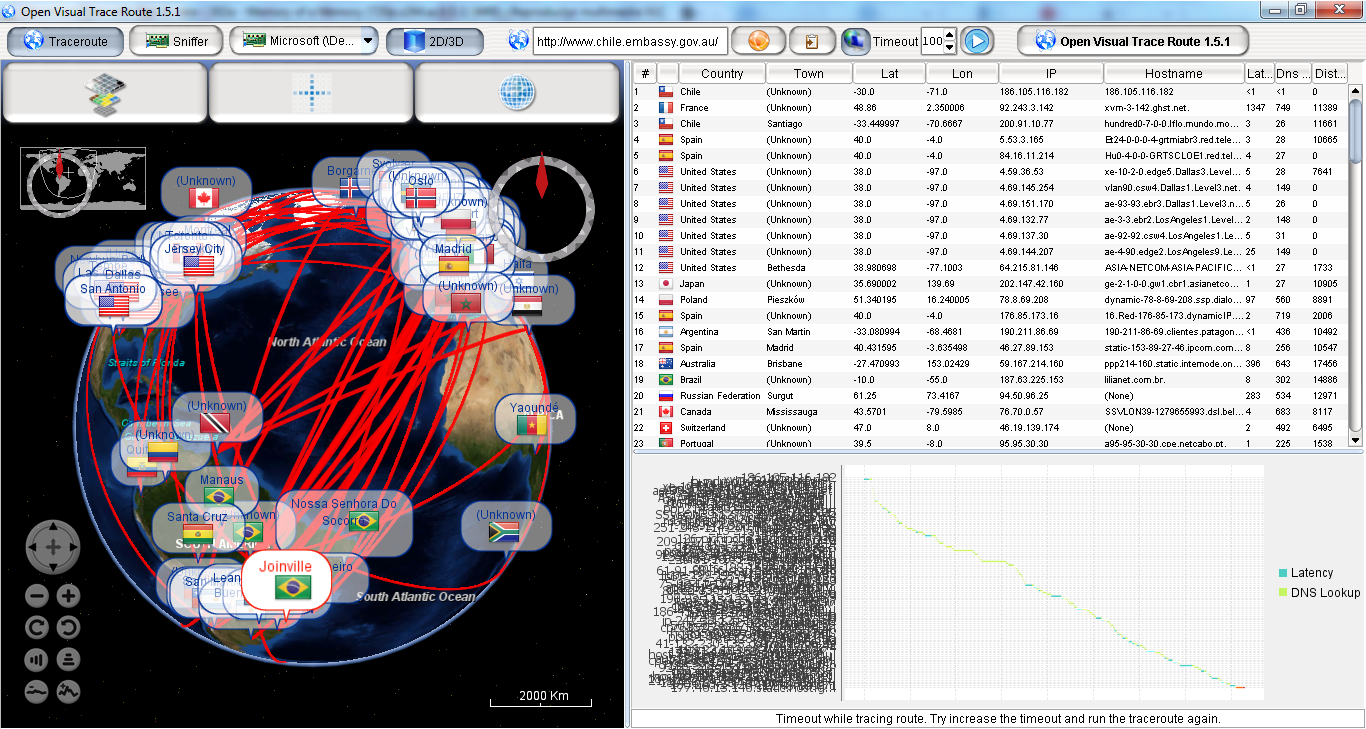
\includegraphics[width=\textwidth]{traceroute_australia.png}
\caption{Trace Route de chile.embassy.gov.au}
\label{fig:embajadaChilena}
\end{figure}  

\end{description}

Cabe notar que los saltos mostrados no son siempre iguales, dependen de varios factores, tales como la hora a la que se hizo el acceso o el lugar geográfico desde el cual se hizo. El camino tomado por los paquetes se decide por el algoritmo de vector de distancia, el cual será estudiado en la sección siguiente.
\clearpage

\subsection{Tabla de costos de routers}

Se dispone una red con nueve routers, donde el PC desea acceder a los archivos que se encuentran en el servidor, tal como se ve en la siguiente figura:

\begin{figure}[H]
\centering
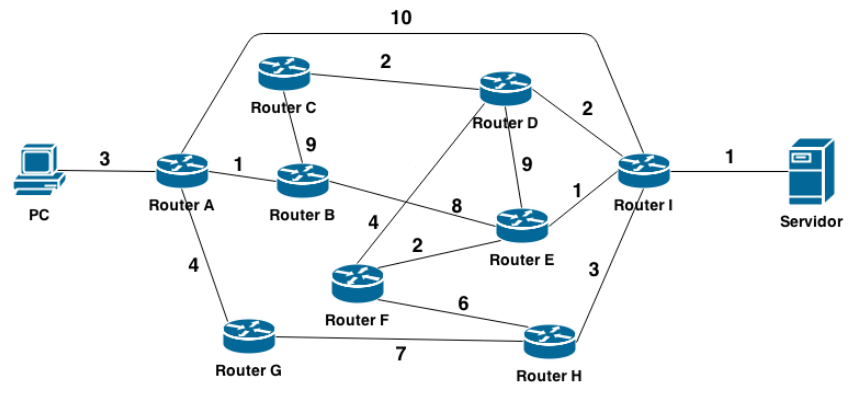
\includegraphics[width=\textwidth]{grafoTarea.png}
\caption{Red de routers}
\label{fig:embajadaChilena}
\end{figure}  

Para este fin, se debe encontrar la ruta más corta para llegar desde el PC al servidor, para lo cual se deben obtener las tablas de costos de los routers, para lo cual se usa el algoritmo vector distancia. Para obtener las tablas de costos de todos los routers mediante el algoritmo vector distancia, debemos realizar una serie de iteraciones. Para el caso de esta experiencia, y solo como a modo de ejemplo ilustrativo, se mostrara la primera inicialización de todas las tablas y se explicara el funcionamiento del algoritmo, para finalmente mostrar como quedan las tablas de costos mediante la implementación en Python del algoritmo vector distancia.

\subsubsection*{Primera Inicialización Tablas De Costos}
Primero se debe inicializar la tabla de costos de cada router de la siguiente manera: Sea x el router al cual se le esta calculando la tabla de costes, en la fila de x se registran los costes para ir de x a todos los demás routers (columnas), si el router es vecino, se registra el costo, si no, se marca como $\infty$ al igual que todas las demás filas que no correspondan al router x.\\
A continuación se muestra la primera iteración para cada tabla de costos de la red ilustrada anteriormente, quedando las siguientes tablas:\\
\\\\
Como se puede ver en la siguiente tabla, la inicialización inicial solo corresponde a los costos de ir desde el router A a sus vecinos directos. Es importante mencionar que ocurre lo mismo con todos los demas.\\\\

Para la tabla del router A:\\
\begin{tabular}{ | c | c | c | c | c | c | c | c | c | c |}
\hline                    
ROUTER A    & A      & B      & C      & D      & E      & F      & G      & H      & I      \\
\hline
        A   & 0      & 1      &$\infty$&$\infty$&$\infty$&$\infty$& 4      &$\infty$& 10     \\
\hline
        B   &$\infty$&$\infty$&$\infty$&$\infty$&$\infty$&$\infty$&$\infty$&$\infty$&$\infty$\\
\hline
        C   &$\infty$&$\infty$&$\infty$&$\infty$&$\infty$&$\infty$&$\infty$&$\infty$&$\infty$\\
\hline
        D   &$\infty$&$\infty$&$\infty$&$\infty$&$\infty$&$\infty$&$\infty$&$\infty$&$\infty$\\
\hline
        E   &$\infty$&$\infty$&$\infty$&$\infty$&$\infty$&$\infty$&$\infty$&$\infty$&$\infty$\\
\hline
        F   &$\infty$&$\infty$&$\infty$&$\infty$&$\infty$&$\infty$&$\infty$&$\infty$&$\infty$\\
\hline
        G   &$\infty$&$\infty$&$\infty$&$\infty$&$\infty$&$\infty$&$\infty$&$\infty$&$\infty$\\
\hline
        H   &$\infty$&$\infty$&$\infty$&$\infty$&$\infty$&$\infty$&$\infty$&$\infty$&$\infty$\\
\hline 
        I   &$\infty$&$\infty$&$\infty$&$\infty$&$\infty$&$\infty$&$\infty$&$\infty$&$\infty$\\
\hline
\end{tabular}
\\\\

Para la tabla del router B:\\
\begin{tabular}{ | c | c | c | c | c | c | c | c | c | c |}
\hline                 
ROUTER B    & A      & B      & C      & D      & E      & F      & G      & H      & I      \\
\hline
        A   &$\infty$&$\infty$&$\infty$&$\infty$&$\infty$&$\infty$&$\infty$&$\infty$&$\infty$\\
\hline
        B   & 1      & 0      & 9      &$\infty$& 8      &$\infty$&$\infty$&$\infty$&$\infty$\\
\hline
        C   &$\infty$&$\infty$&$\infty$&$\infty$&$\infty$&$\infty$&$\infty$&$\infty$&$\infty$\\
\hline
        D   &$\infty$&$\infty$&$\infty$&$\infty$&$\infty$&$\infty$&$\infty$&$\infty$&$\infty$\\
\hline
        E   &$\infty$&$\infty$&$\infty$&$\infty$&$\infty$&$\infty$&$\infty$&$\infty$&$\infty$\\
\hline
        F   &$\infty$&$\infty$&$\infty$&$\infty$&$\infty$&$\infty$&$\infty$&$\infty$&$\infty$\\
\hline
        G   &$\infty$&$\infty$&$\infty$&$\infty$&$\infty$&$\infty$&$\infty$&$\infty$&$\infty$\\
\hline
        H   &$\infty$&$\infty$&$\infty$&$\infty$&$\infty$&$\infty$&$\infty$&$\infty$&$\infty$\\
\hline 
        I   &$\infty$&$\infty$&$\infty$&$\infty$&$\infty$&$\infty$&$\infty$&$\infty$&$\infty$\\
\hline
\end{tabular}
\\\\
Para la tabla del router C:\\
\begin{tabular}{ | c | c | c | c | c | c | c | c | c | c | c | c |}
\hline                 
ROUTER C    & A      & B      & C      & D      & E      & F      & G      & H      & I      \\
\hline
        A   &$\infty$&$\infty$&$\infty$&$\infty$&$\infty$&$\infty$&$\infty$&$\infty$&$\infty$\\
\hline
        B   &$\infty$&$\infty$&$\infty$&$\infty$&$\infty$&$\infty$&$\infty$&$\infty$&$\infty$\\
\hline
        C   &$\infty$& 9      & 0      & 2      &$\infty$&$\infty$&$\infty$&$\infty$&$\infty$\\
\hline
        D   &$\infty$&$\infty$&$\infty$&$\infty$&$\infty$&$\infty$&$\infty$&$\infty$&$\infty$\\
\hline
        E   &$\infty$&$\infty$&$\infty$&$\infty$&$\infty$&$\infty$&$\infty$&$\infty$&$\infty$\\
\hline
        F   &$\infty$&$\infty$&$\infty$&$\infty$&$\infty$&$\infty$&$\infty$&$\infty$&$\infty$\\
\hline
        G   &$\infty$&$\infty$&$\infty$&$\infty$&$\infty$&$\infty$&$\infty$&$\infty$&$\infty$\\
\hline
        H   &$\infty$&$\infty$&$\infty$&$\infty$&$\infty$&$\infty$&$\infty$&$\infty$&$\infty$\\
\hline 
        I   &$\infty$&$\infty$&$\infty$&$\infty$&$\infty$&$\infty$&$\infty$&$\infty$&$\infty$\\
\hline
\end{tabular}
\\\\
\clearpage
Para la tabla del router D:\\
\begin{tabular}{ | c | c | c | c | c | c | c | c | c | c |}
\hline                 
ROUTER D    & A      & B      & C      & D      & E      & F      & G      & H      & I      \\
\hline
        A   &$\infty$&$\infty$&$\infty$&$\infty$&$\infty$&$\infty$&$\infty$&$\infty$&$\infty$\\
\hline
        B   &$\infty$&$\infty$&$\infty$&$\infty$&$\infty$&$\infty$&$\infty$&$\infty$&$\infty$\\
\hline
        C   &$\infty$&$\infty$&$\infty$&$\infty$&$\infty$&$\infty$&$\infty$&$\infty$&$\infty$\\
\hline
        D   &$\infty$&$\infty$& 2      & 0      & 9      & 4      &$\infty$&$\infty$& 2      \\
\hline
        E   &$\infty$&$\infty$&$\infty$&$\infty$&$\infty$&$\infty$&$\infty$&$\infty$&$\infty$\\
\hline
        F   &$\infty$&$\infty$&$\infty$&$\infty$&$\infty$&$\infty$&$\infty$&$\infty$&$\infty$\\
\hline
        G   &$\infty$&$\infty$&$\infty$&$\infty$&$\infty$&$\infty$&$\infty$&$\infty$&$\infty$\\
\hline
        H   &$\infty$&$\infty$&$\infty$&$\infty$&$\infty$&$\infty$&$\infty$&$\infty$&$\infty$\\
\hline 
        I   &$\infty$&$\infty$&$\infty$&$\infty$&$\infty$&$\infty$&$\infty$&$\infty$&$\infty$\\
\hline
\end{tabular}
\\\\
Para la tabla del router E:\\
\begin{tabular}{ | c | c | c | c | c | c | c | c | c | c |}
\hline                 
ROUTER E    & A      & B      & C      & D      & E      & F      & G      & H      & I      \\
\hline
        A   &$\infty$&$\infty$&$\infty$&$\infty$&$\infty$&$\infty$&$\infty$&$\infty$&$\infty$\\
\hline
        B   &$\infty$&$\infty$&$\infty$&$\infty$&$\infty$&$\infty$&$\infty$&$\infty$&$\infty$\\
\hline
        C   &$\infty$&$\infty$&$\infty$&$\infty$&$\infty$&$\infty$&$\infty$&$\infty$&$\infty$\\
\hline
        D   &$\infty$&$\infty$&$\infty$&$\infty$&$\infty$&$\infty$&$\infty$&$\infty$&$\infty$\\
\hline
        E   &$\infty$& 8      &$\infty$& 9      & 0      & 2      &$\infty$&$\infty$& 1      \\
\hline
        F   &$\infty$&$\infty$&$\infty$&$\infty$&$\infty$&$\infty$&$\infty$&$\infty$&$\infty$\\
\hline
        G   &$\infty$&$\infty$&$\infty$&$\infty$&$\infty$&$\infty$&$\infty$&$\infty$&$\infty$\\
\hline
        H   &$\infty$&$\infty$&$\infty$&$\infty$&$\infty$&$\infty$&$\infty$&$\infty$&$\infty$\\
\hline 
        I   &$\infty$&$\infty$&$\infty$&$\infty$&$\infty$&$\infty$&$\infty$&$\infty$&$\infty$\\
\hline
\end{tabular}
\\\\
Para la tabla del router F:\\
\begin{tabular}{ | c | c | c | c | c | c | c | c | c | c |}
\hline                 
ROUTER F    & A      & B      & C      & D      & E      & F      & G      & H      & I      \\
\hline
        A   &$\infty$&$\infty$&$\infty$&$\infty$&$\infty$&$\infty$&$\infty$&$\infty$&$\infty$\\
\hline
        B   &$\infty$&$\infty$&$\infty$&$\infty$&$\infty$&$\infty$&$\infty$&$\infty$&$\infty$\\
\hline
        C   &$\infty$&$\infty$&$\infty$&$\infty$&$\infty$&$\infty$&$\infty$&$\infty$&$\infty$\\
\hline
        D   &$\infty$&$\infty$&$\infty$&$\infty$&$\infty$&$\infty$&$\infty$&$\infty$&$\infty$\\
\hline
        E   &$\infty$&$\infty$&$\infty$&$\infty$&$\infty$&$\infty$&$\infty$&$\infty$&$\infty$\\
\hline
        F   &$\infty$&$\infty$&$\infty$& 4      & 2      & 0      &$\infty$& 6      &$\infty$\\
\hline
        G   &$\infty$&$\infty$&$\infty$&$\infty$&$\infty$&$\infty$&$\infty$&$\infty$&$\infty$\\
\hline
        H   &$\infty$&$\infty$&$\infty$&$\infty$&$\infty$&$\infty$&$\infty$&$\infty$&$\infty$\\
\hline 
        I   &$\infty$&$\infty$&$\infty$&$\infty$&$\infty$&$\infty$&$\infty$&$\infty$&$\infty$\\
\hline
\end{tabular}
\\\\
Para la tabla del router G:\\
\begin{tabular}{ | c | c | c | c | c | c | c | c | c | c |}
\hline                 
ROUTER G    & A      & B      & C      & D      & E      & F      & G      & H      & I      \\
\hline
        A   &$\infty$&$\infty$&$\infty$&$\infty$&$\infty$&$\infty$&$\infty$&$\infty$&$\infty$\\
\hline
        B   &$\infty$&$\infty$&$\infty$&$\infty$&$\infty$&$\infty$&$\infty$&$\infty$&$\infty$\\
\hline
        C   &$\infty$&$\infty$&$\infty$&$\infty$&$\infty$&$\infty$&$\infty$&$\infty$&$\infty$\\
\hline
        D   &$\infty$&$\infty$&$\infty$&$\infty$&$\infty$&$\infty$&$\infty$&$\infty$&$\infty$\\
\hline
        E   &$\infty$&$\infty$&$\infty$&$\infty$&$\infty$&$\infty$&$\infty$&$\infty$&$\infty$\\
\hline
        F   &$\infty$&$\infty$&$\infty$&$\infty$&$\infty$&$\infty$&$\infty$&$\infty$&$\infty$\\
\hline
        G   & 4      &$\infty$&$\infty$&$\infty$&$\infty$&$\infty$& 0      & 7      &$\infty$\\
\hline
        H   &$\infty$&$\infty$&$\infty$&$\infty$&$\infty$&$\infty$&$\infty$&$\infty$&$\infty$\\
\hline 
        I   &$\infty$&$\infty$&$\infty$&$\infty$&$\infty$&$\infty$&$\infty$&$\infty$&$\infty$\\
\hline
\end{tabular}
\\\\
Para la tabla del router H:\\
\begin{tabular}{ | c | c | c | c | c | c | c | c | c | c | c | c |}
\hline                 
ROUTER H    & A      & B      & C      & D      & E      & F      & G      & H      & I      \\
\hline
        A   &$\infty$&$\infty$&$\infty$&$\infty$&$\infty$&$\infty$&$\infty$&$\infty$&$\infty$\\
\hline
        B   &$\infty$&$\infty$&$\infty$&$\infty$&$\infty$&$\infty$&$\infty$&$\infty$&$\infty$\\
\hline
        C   &$\infty$&$\infty$&$\infty$&$\infty$&$\infty$&$\infty$&$\infty$&$\infty$&$\infty$\\
\hline
        D   &$\infty$&$\infty$&$\infty$&$\infty$&$\infty$&$\infty$&$\infty$&$\infty$&$\infty$\\
\hline
        E   &$\infty$&$\infty$&$\infty$&$\infty$&$\infty$&$\infty$&$\infty$&$\infty$&$\infty$\\
\hline
        F   &$\infty$&$\infty$&$\infty$&$\infty$&$\infty$&$\infty$&$\infty$&$\infty$&$\infty$\\
\hline
        G   &$\infty$&$\infty$&$\infty$&$\infty$&$\infty$&$\infty$&$\infty$&$\infty$&$\infty$\\
\hline
        H   &$\infty$&$\infty$&$\infty$&$\infty$&$\infty$& 6      & 7      & 0      & 3      \\
\hline 
        I   &$\infty$&$\infty$&$\infty$&$\infty$&$\infty$&$\infty$&$\infty$&$\infty$&$\infty$\\
\hline
\end{tabular}
\\\\

Para la tabla del router I:\\
\begin{tabular}{ | c | c | c | c | c | c | c | c | c | c |}
\hline                 
ROUTER I    & A      & B      & C      & D      & E      & F      & G      & H      & I      \\
\hline
        A   &$\infty$&$\infty$&$\infty$&$\infty$&$\infty$&$\infty$&$\infty$&$\infty$&$\infty$\\
\hline
        B   &$\infty$&$\infty$&$\infty$&$\infty$&$\infty$&$\infty$&$\infty$&$\infty$&$\infty$\\
\hline
        C   &$\infty$&$\infty$&$\infty$&$\infty$&$\infty$&$\infty$&$\infty$&$\infty$&$\infty$\\
\hline
        D   &$\infty$&$\infty$&$\infty$&$\infty$&$\infty$&$\infty$&$\infty$&$\infty$&$\infty$\\
\hline
        E   &$\infty$&$\infty$&$\infty$&$\infty$&$\infty$&$\infty$&$\infty$&$\infty$&$\infty$\\
\hline
        F   &$\infty$&$\infty$&$\infty$&$\infty$&$\infty$&$\infty$&$\infty$&$\infty$&$\infty$\\
\hline
        G   &$\infty$&$\infty$&$\infty$&$\infty$&$\infty$&$\infty$&$\infty$&$\infty$&$\infty$\\
\hline
        H   &$\infty$&$\infty$&$\infty$&$\infty$&$\infty$&$\infty$&$\infty$&$\infty$&$\infty$\\
\hline 
        I   & 10     &$\infty$&$\infty$& 2      & 1      &$\infty$&$\infty$& 3      & 0      \\
\hline
\end{tabular}
\subsubsection*{Calculo Tablas De Costos (Script Python)}
Para poder obtener las tablas de costos de cada router se creó un programa en Python que se encarga de obtener las tablas de costos asociadas a cada router. El funcionamiento del programa es el siguiente:

Primero se definieron los parámetros básicos para trabajar, dígase la inicialización de los datos básicos, como son los adyacentes a cada router con sus costos, y otros parámetros auxiliares, como se pueden apreciar a continuación:

\begin{python}
inf=9999999
adyA=[0,1,inf,inf,inf,inf,4,inf,10]
adyB=[1,0,9,inf,8,inf,inf,inf,inf]
adyC=[inf,9,0,2,inf,inf,inf,inf,inf]
adyD=[inf,inf,2,0,9,4,inf,inf,2]
adyE=[inf,8,inf,9,0,2,inf,inf,1]
adyF=[inf,inf,inf,4,2,0,inf,6,inf]
adyG=[4,inf,inf,inf,inf,inf,0,7,inf]
adyH=[inf,inf,inf,inf,inf,6,7,0,3]
adyI=[10,inf,inf,2,1,inf,inf,3,0]	
adyacentes=[adyA,adyB,adyC, ... ,adyH,adyI]
lista=[0,1,2,3,4,5,6,7,8]
costosAct=[]
costosSig=[]
valor_act=[0,0,0,0,0,0,0,0,0]
\end{python}

Como se puede observar, $adyacentes$ contiene toda la información acerca de las conexiones entre los routers y los costos entre ellos, tal como seria una representación de una matriz de adyacencia. En las variables $costosAct$ y $costosSig$ se almacenaran las tablas de costos, una para almacenar el estado actual de las tablas y otra para el estado siguiente.\\
Luego de tener la información base precargada, se procedió a calcular las tablas de costo iniciales, esto mediante la siguiente función:
\begin{python}

def init():
    cpyAdy=copy.deepcopy(adyacentes)
    tcost=[[],[],[],[],[],[],[],[],[]]
    vector=[inf,inf,inf,inf,inf,inf,inf,inf,inf]
    for i in lista:
        for j in lista:
            if i==j:
                tcost[j].append(cpyAdy[j])
            else:
                tcost[j].append(vector)
    return tcost
\end{python}

Posteriormente, se procedió a definir el método $dxy$, que es el que se encarga de calcular los costos aproximados $d_x(y)$ mediante el algoritmo de Bellman Ford, cuya implementación se muestra a continuación:

\begin{python}
def dxy(x,y,costosAct):
    costosVecinos=[]
    vecinos=[]
    costo=0
    dvy=0
    for i in lista:
        if adyacentes[x][i]<inf:
            vecinos.append(0+i)
        for ady in vecinos:
            costo=0 + adyacentes[x][ady]
            dvy=0 + costosAct[ady][ady][y]
            costosVecinos.append(costo+dvy)
    return menor_lista(costosVecinos)
\end{python}

Finalmente, se implementó el método $vectorDist$, cuyo código es:

\begin{python}
def vectorDist(CA,CS,valor_act):
    vecinos=[]
    for i in range(9):
        for j in range(9):
            valor=dxy(i,j,CA)
            if valor<CA[i][i][j] and valor<CS[i][i][j]:
                CS[i][i][j]=valor
                valor_act[i]=1
            for k in lista:
                if adyacentes[i][k]<inf and adyacentes[i][k]>0:
                    vecinos.append(0+k)
            for v in vecinos:
                CS[i][v]=copy.deepcopy(CA[v][v])
    for l in lista:
        CA[l]=copy.deepcopy(CS[l])
    continuar=sumalist(valor_act)
    aux=copy.deepcopy(valor_act)
    while(continuar>0):
        for i in lista:
            v=[]#no hay vecinos
            valor_act[i]=0
            for k in lista:
                if adyacentes[i][k]<inf and adyacentes[i][k]>0:
                    vecinos.append(0+k)
            for v in vecinos:
                if aux[v]>0:
                    CS[i][v]=copy.deepcopy(CA[v][v])
                    for j in lista:
                        valor=dxy(i,j,CA)
                        if valor<CA[i][i][j] and valor<CS ... :
                            CS[i][i][j]=valor
                            valor_act[i]=valor_act[i]+1
        for l in lista:
            CA[l]=copy.deepcopy(CS[l])
        continuar=sumalist(valor_act)
        aux=copy.deepcopy(valor_act)
\end{python}

La función anterior funciona de la siguiente forma:

\begin{itemize}

\item Primero inicializa los datos de las tablas de costos iniciales, y registra que todos los nodos se han actualizado.
\item Luego itera nodo por nodo revisando si sus vecinos se han modificado, de ser así, entonces actualiza los $D_v$ (vector distancia de sus vecinos) en su tabla de costos y calcula si con la nueva información su vector de distancias cambia, de ser efectivo registra que se modifico, y se continua iterando con los otros routers. Así sucesivamente hasta que pase una iteración en que ningún router modifique su tabla de costos.
\end{itemize}

Finalmente, el algoritmo genera las tablas de costos de todos los routers, las cuales resultaron ser las siguientes:

\begin{figure}[H]
\centering
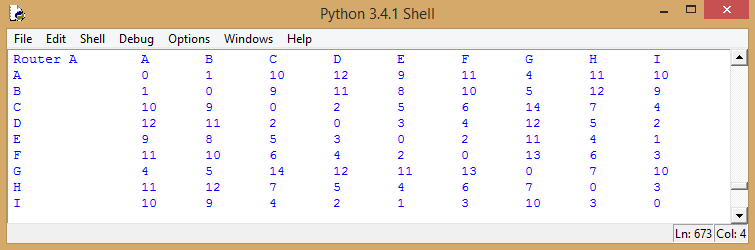
\includegraphics[width=\textwidth]{p21.png}
\caption{Tabla de costos final del router A}
\label{fig:Tabla de costos}
\end{figure} 

\begin{figure}[H]
\centering
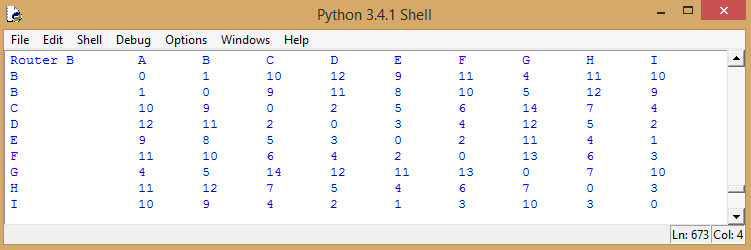
\includegraphics[width=\textwidth]{p22.png}
\caption{Tabla de costos final del router B}
\label{fig:Tabla de costos}
\end{figure}

\begin{figure}[H]
\centering
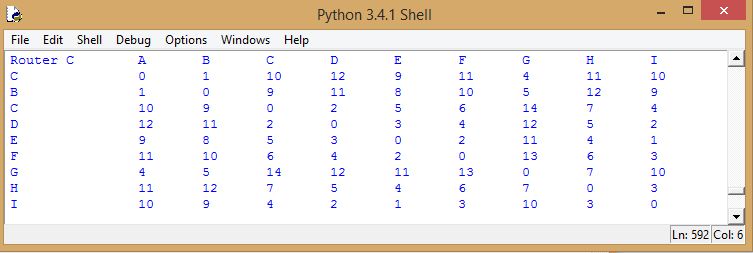
\includegraphics[width=\textwidth]{p23.png}
\caption{Tabla de costos final del router C}
\label{fig:Tabla de costos}
\end{figure}

\begin{figure}[H]
\centering
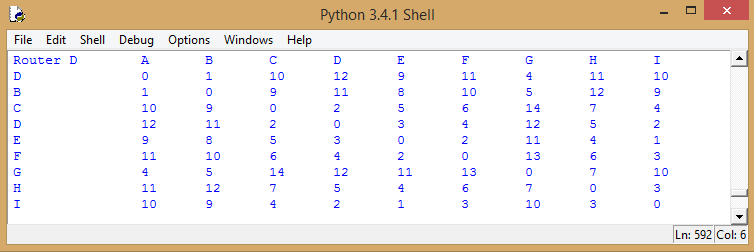
\includegraphics[width=\textwidth]{p24.png}
\caption{Tabla de costos final del router D}
\label{fig:Tabla de costos}
\end{figure}

\begin{figure}[H]
\centering
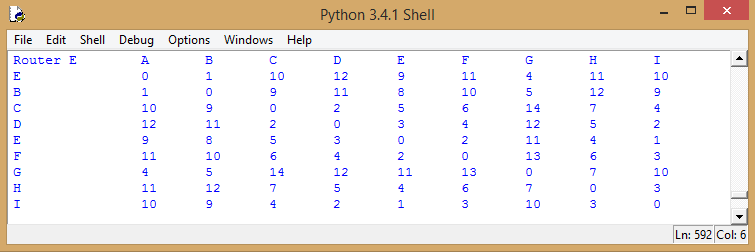
\includegraphics[width=\textwidth]{p25.png}
\caption{Tabla de costos final del router E}
\label{fig:Tabla de costos}
\end{figure}

\begin{figure}[H]
\centering
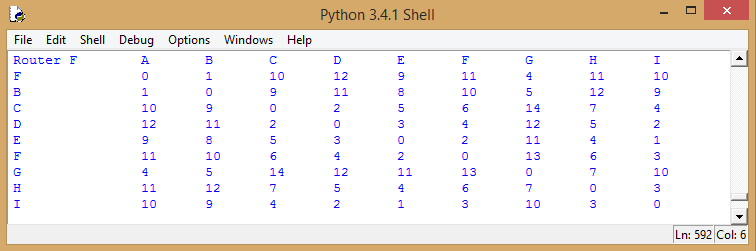
\includegraphics[width=\textwidth]{p26.png}
\caption{Tabla de costos final del router F}
\label{fig:Tabla de costos}
\end{figure}

\begin{figure}[H]
\centering
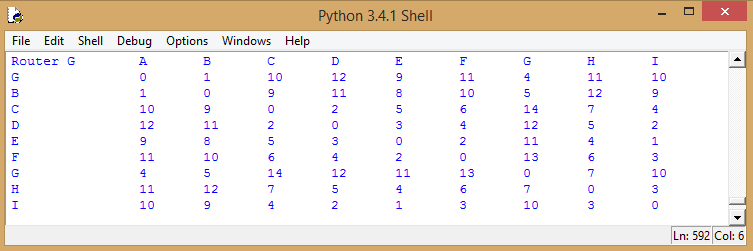
\includegraphics[width=\textwidth]{p27.png}
\caption{Tabla de costos final del router G}
\label{fig:Tabla de costos}
\end{figure}

\begin{figure}[H]
\centering
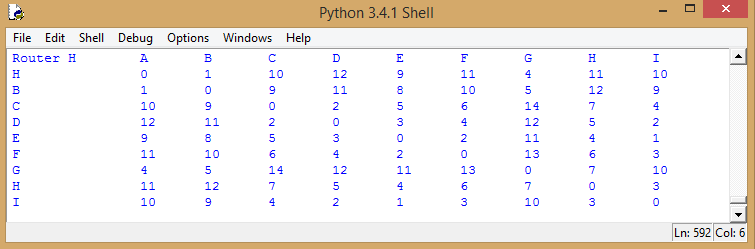
\includegraphics[width=\textwidth]{p28.png}
\caption{Tabla de costos final del router H}
\label{fig:Tabla de costos}
\end{figure}

\begin{figure}[H]
\centering
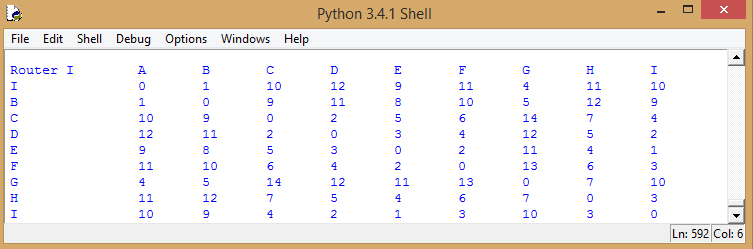
\includegraphics[width=\textwidth]{p29.png}
\caption{Tabla de costos final del router I}
\label{fig:Tabla de costos}
\end{figure}

Como se puede observar, al final de las iteraciones cada router conoce los costos de todos los demás, obteniéndose la misma tabla para cada router, aun cuando los routers solo se intercambiaban información con sus vecinos.

\subsection{Tabla de costo de routers en caso de modificación de conexiones}
Para esta parte, se estudia el caso en que se corta la conexión entre dos routers, en este caso entre router H y router I. Para estudiar este caso, se creó una versión adaptada de la función $vectorDist$, que elimina la conexión para el arreglo de routers, cuya implementación se muestra a continuación:

\begin{python}
def vectorDistInt(CA,CS,valor_act):
    vecinos=[]
    CA[7][7][8]=inf
    CA[8][8][7]=inf
    CS[7][7][8]=inf
    CS[8][8][7]=inf
    adyH[8]=inf
    adyI[7]=inf
    adyacentes=[adyA,adyB,adyC, ... ,adyH,adyI]
    valor_act[7]=1
    valor_act[8]=1
    #ahora iteramos nuevamente
    continuar=sumalist(valor_act)
    aux=copy.deepcopy(valor_act)
    while(continuar>0):
        for i in lista:
            v=[]
            valor_act[i]=0
            for k in lista:#determinamos los vecinos a i
                if adyacentes[i][k]<inf and adyacentes[i][k]>0:
                    vecinos.append(0+k)#guardarid vecinos de i
            for v in vecinos:#para cada vecino ver si se modifico
                if aux[v]>0:#si se modifico
                    CS[i][v]=copy.deepcopy(CA[v][v])
                    for j in lista:
                        valor=dxy(i,j,CA)
                        if valor<CA[i][i][j] and valor<CS[i][i][j]:
                            CS[i][i][j]=valor
                            valor_act[i]=valor_act[i]+1
        for l in lista:
            CA[l]=copy.deepcopy(CS[l])
        continuar=sumalist(valor_act)
        aux=copy.deepcopy(valor_act)

\end{python}

Finalmente, el algoritmo entonces genera las tablas de costos de todos los routers al romperse el enlace, que análogamente al caso anterior presentan todos los mismos valores, razón por la cual solo adjuntaremos una en este caso:

\begin{figure}[H]
\centering
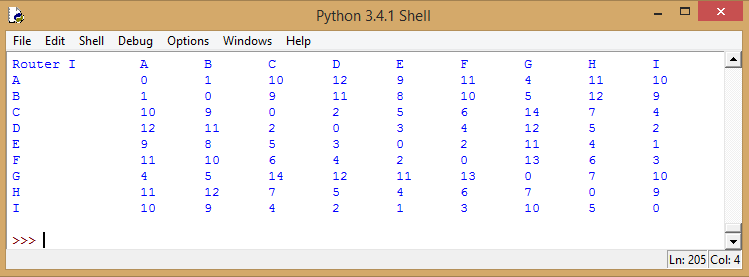
\includegraphics[width=\textwidth]{p31.png}
\caption{Tabla de costos final del router I con enlace a H roto}
\label{fig:Tabla de costos}
\end{figure} 

\section{Conclusión}

Como se pudo ver, el algoritmo vector distancia, además de ayudar a encontrar la ruta más corta para el envío de paquetes, también le da robustez a la las conexiones, ya que en caso de cortes de conexiones, como fue visto en la sección 2.3, los routers informan a sus vecinos los cambios de topología, lo cual es usado para encontrar rápidamente una nueva ruta optima. Las conexiones intercontinentales funcionan de igual forma, ya que en caso de cortes de cable, se calcula rápidamente un nuevo camino para el envío de paquetes, así no se deja a continentes enteros sin internet en caso de contratiempos.

\bibliographystyle{plain}
\clearpage
\bibliography{references}
\end{document}
